En este capítulo se expone la arquitectura final del sistema propuesto, así como
el proceso de desarrollo del mismo en cada una de las partes y como todas estas
funcionan en conjunto. 

\section{Arquitectura del sistema} El sistema final consta de una
serie de módulos, serán referidos como tal pese a ser más parecidos a
herramientas que a módulos, a diferencia de como se esperaría en un producto
interconectado.

La finalidad deseada es la creación de un modelo de Aprendizaje Profundo que sea
capaz de, dado un texto, asignar los objetivos de desarrollo sostenible
relacionados con los temas tratados en el mismo. 

En este tipo de tareas se requiere de tres funcionalidades fundamentales, la
extracción y análisis de datos, la creación y validación de modelos y una forma
de usarlos fácil y eficiente.

Las arquitecturas de estas funcionalidades están representadas en los siguientes
diagramas, por motivos de claridad se muestran por separado. Todas ellas
funcionan al rededor de la base de datos. Esta hace la función de piedra angular
de la arquitectura, por lo que es a través de este elemento por el que se puede
ver la interacción entre los diferentes módulos:

\subsection{Recogida de datos}
\begin{figure}[H]
    \centering
    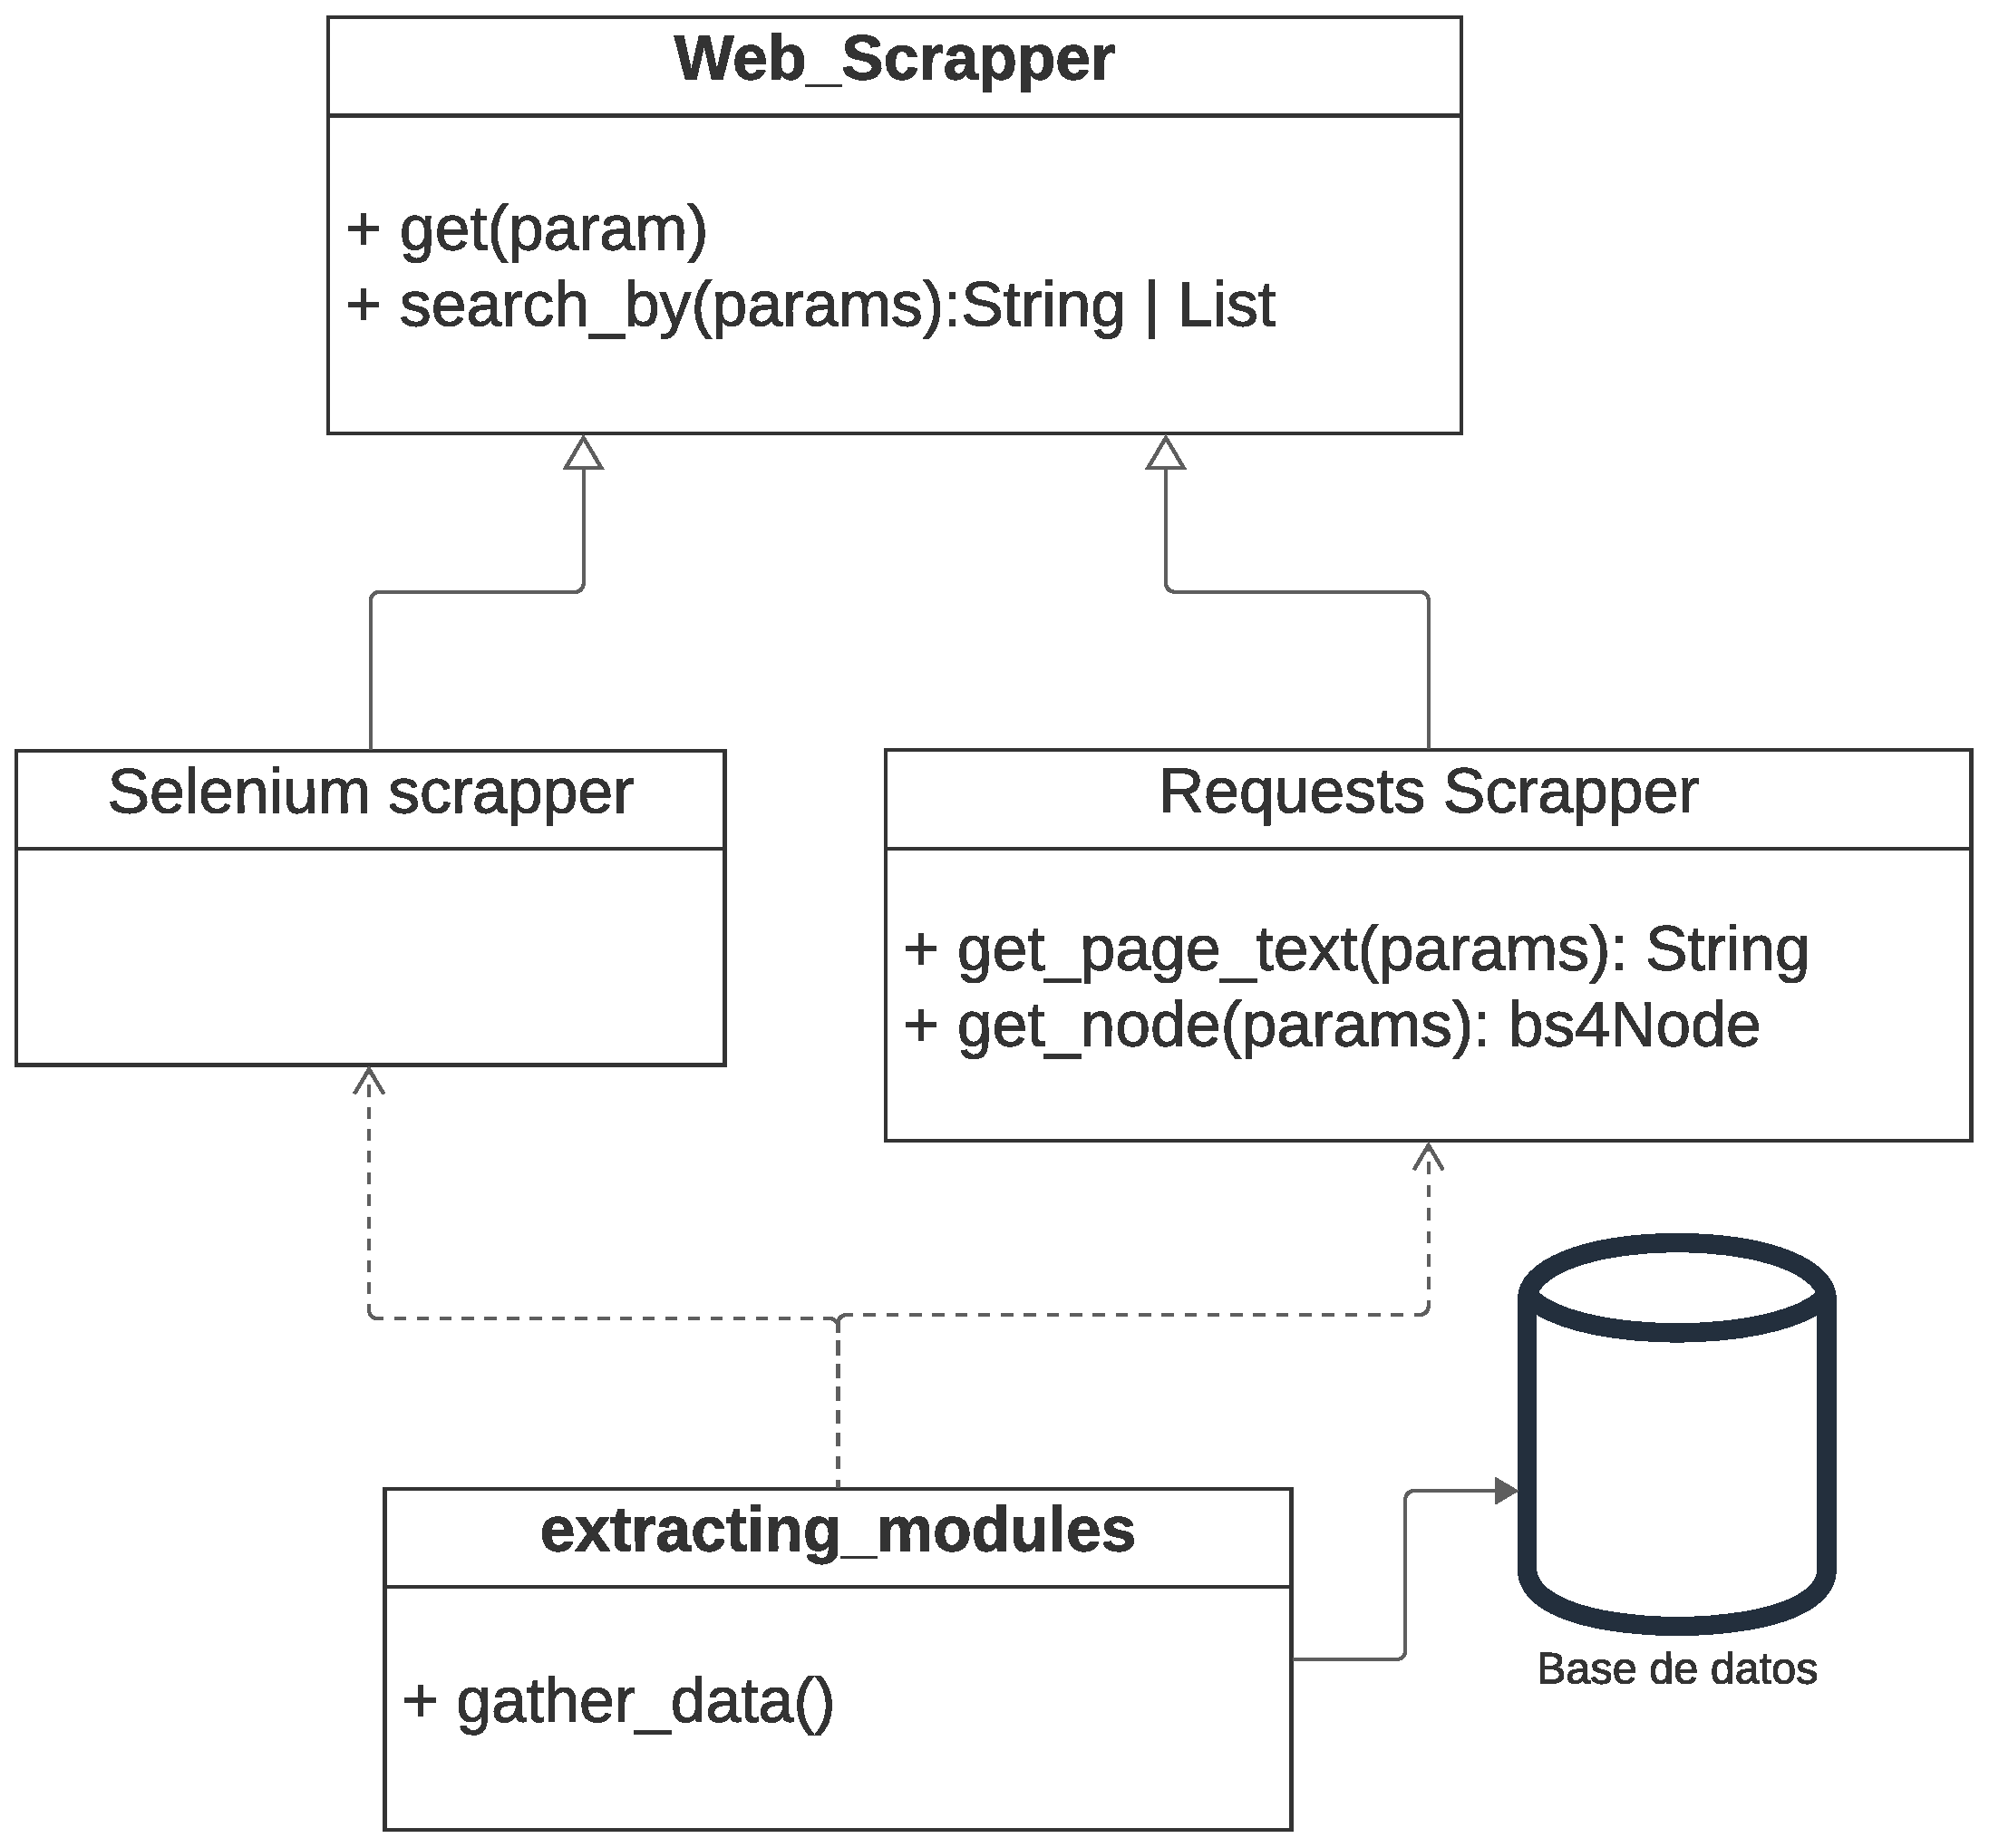
\includegraphics[width=0.65\textwidth]{data_gathering}
    \captionsetup{justification=centering}
    \caption{Diagrama UML de la arquitectura de recogida de datos}
    \label{fig: Diagrama UML de la arquitectura de recogida de datos}
\end{figure}

Para el desarrollo de este sistema se han creado los siguientes módulos:

\subsubsection{Módulo de WebScrapping} Después de una exhaustiva investigación se llegó a la
conclusión de que no existe ninguna base de datos extensa con textos etiquetados
relacionados con los \gls{ODSg}, es por esto que fue
necesario el desarrollo de un módulo de \textit{Web Scrapping}. Este sirve únicamente como
herramienta para facilitar la extracción de datos, son otros módulos los que lo
usan para implementar la lógica necesaria para realizar la extracción.

La arquitectura de este módulo es sencilla desde fuera pero con múltiples
funcionalidades, como se definió en el estado del arte existen dos métodos para
realizar esta extracción, es por esto por lo que se creó una clase padre con el
esqueleto de una herramienta de este tipo, esta es sencilla constando de dos
métodos diferentes: 

\begin{itemize}
    \item Un método \textit{get} que sirve para especificar la página web de la que
    extraer los datos ya que ambos tienen como primer paso acceder a la página
    \item Un método \textit{search\_by} que sirve para la extracción de los datos. 
\end{itemize}

En la clase padre estos métodos están vacíos, contacto únicamente con un
comentario explicando la funcionalidad deseada.

Las dos clases creadas son las siguientes:
\paragraph{requests\_scrapper} Esta primera clase implementa el tipo de extracción más
rápido, la extracción del código fuente devuelto por la petición \gls{httpa}
directamente, sin ningún tipo de interacción. Como para la extracción de textos
habitualmente no se requiere de interacción es, de las dos clases, la más
desarrollada. 

Implementa un total de cuatro métodos, los dos métodos definidos en la clase
padre y dos adicionales, estos son: 

\begin{itemize}
    \item \textbf{get}: Método definido en la clase padre,
    realiza mediante la librería \textit{requests} una petición \gls{httpa} a la página
    especificada, incluyendo en esta una serie de cabeceras para que el destinatario
    no rechace la conexión. Posteriormente hace uso de la librería \textit{BeautifulSoup4}
    para interpretar el código \gls{htmla} y poder extraer datos de la página de
    una manera sencilla, especificando atributos de los diferentes elementos que
    conforman la página. 
    \item \textbf{get\_page\_text}: este método tiene una funcionalidad muy
    simple, únicamente devuelve el texto plano incluido en la página. Gracias a
    interpretar el código con \textit{BeautifulSoup4} esta tarea es muy fácil ya que el
    objeto creado por esta librería incluye un atributo el cual contiene el
    texto de toda la página 
    
    
    \item \textbf{get\_node}: la funcionalidad de este método es parecida a la de get
    pero en vez de especificar la página en la que buscar se especifica un elemento
    de la página web. Esto reduce el entorno de búsqueda al contenido de un solo
    nodo de la página web. Esto es necesario en algunos casos ya que si el nodo
    que contiene el texto a extraer no tiene ningún parámetro que lo identifique
    unívocamente, esta identificación se puede realizar en un nodo superior que
    lo contenga, de esta manera es más probable que algún atributo pueda ser
    usado para identificarlo. 

    \item \textbf{search\_by}: este es el método más completo y complejo de los
    cuatro desarrollados ya que realiza la función de extracción de texto. Para
    la extracción es necesario identificar el nodo \gls{htmla} que contiene el texto,
    esto se puede realizar de 5 maneras diferentes: por clase, id, xpath,
    custom, tag. 
    \begin{itemize}
        \item Por clase: esta es de todas la más útil pero a la vez la más
        difícil de utilizar ya que una clase puede identificar a varios nodos,
        de manera que la búsqueda puede resultar en un error o en la extracción
        del texto equivocado. Esto se soluciona con una serie de filtros. El
        primero de ellos determina si se desea una extracción múltiple, es
        decir, el texto de todos los nodos que contengan la clase dada o solo
        uno, si se quieren todos simplemente de identificar, se extrae el texto
        y este se devuelve. Si se quiere el texto de uno de ellos es necesario
        indicar el índice del nodo a extraer, este indica su posición en la
        lista de todos los nodos que contienen la clase dada, esto se puede
        hacer de varias maneras, si se sabe que solo un nodo de la página tiene
        la clase indicada no se proporciona un índice y se extrae el texto, si
        este no es el caso pero se sabe que el resto de nodos no contienen
        ningún tipo de texto se puede extraer el del primer nodo que si tenga y
        si esto tampoco se puede afirmar habrá que proporcionar la posición
        deseada. 
        
        \item Por ID: la más sencilla de todas pero a su vez la menos útil,
        simplemente se proporciona el ID del nodo objetivo y se extrae el texto
        de este. Este método no resulta muy útil ya que en la mayoría de los
        casos los nodos no cuentan con IDs, de hecho se codificó la opción para
        usarlos pero nunca se desarrolló porque no se encontró ningún nodo con
        ID. 
    
        \item Por TAG: TAG es el tipo de nodo de \gls{htmla} (lo que se encuentra entre
        <>),  esta funcionalidad es útil cuando se reduce el espacio de búsqueda
        usando \textit{get\_node()} ya que en ocasiones se da el caso de que el nodo que
        contiene el texto no tiene ningún atributo asociado pero alguno de sus
        nodos padre si y es probable que el tag del nodo deseado si lo
        identifique unívocamente en el espacio de dentro del padre debido a la
        existencia de nodos específicos para incluir texto. 
    
        \item Por XPATH: esta funcionalidad se usa como último recurso, cuando
        el nodo no se puede identificar por ningún otro método. XPATH es la
        posición absoluta del nodo deseado dentro de la página, del tipo
        ``/html/body/div[1]/div/``, donde se ponen en orden todos los nodos padres
        separados por “/” y si estos contienen más de un hijo la posición del
        siguiente. Esta funcionalidad es potente ya que siempre va a identificar
        a un nodo de manera unívoca pero es altamente susceptible a cambios en
        el código fuente. De todas formas, si se desea extraer datos de
        múltiples nodos y estos siguen algún tipo de patrón dentro del código
        fuente, esta es una funcionalidad extremadamente útil, permitiendo
        iterar por todos los elementos dentro de un nodo. 
    \end{itemize}
    Adicionalmente, este método cuenta con dos opciones extra: la opción de
    filtrar el texto que devuelve, eliminando caracteres especiales, comillas,
    comas, saltos de línea dobles y codificando el texto en \gls{ASCIIg} (\gls{ASCIIg}) eliminando todos
    aquellos caracteres que den error y volviéndolo a codificar en \gls{UTF-8g} (\gls{UTF-8a}) y la opción
    de que en vez de devolver el texto se devuelva el nodo seleccionado por si se
    quiere extraer algún otro tipo de información no textual de este o si se quiere
    usar para reducir el espacio de búsqueda.
\end{itemize}


\paragraph{selenium\_scrapper} Esta segunda clase implementa el otro tipo de extracción,
aquella en la cual se interactúa con la página por medio de un navegador para
extraer los datos deseados. Esto se realiza haciendo uso de las librerías de
\textit{Selenium} para implementar toda la lógica de interacción y extracción y
\textit{chromedriver\_autoinstaller} para la instalación del driver web, necesario para
permitir que el programa haga uso de un navegador. Esta clase está menos
desarrollada que la otra debido a que se ha usado en menos ocasiones por lo que
se han identificado menos funcionalidades que implementar, es por esto que
cuenta únicamente con los métodos definidos por la clase padre: 

\begin{itemize}
    \item \textbf{get}: instancia el driver de chrome en la página web deseada. 
    \item \textbf{search\_by}: este método es similar al implementado en la otra clase
    pero con una crucial diferencia, en ningún caso devuelve el texto del nodo
    si no que devuelve el nodo en sí ya que de esta manera se puede interactuar
    con la página realizando acciones como hacer click o escribir. De hecho su principal
    función ha sido extraer las direcciones web de diversos artículos de los
    cuales posteriormente se ha extraído el texto usando la otra clase. 
\end{itemize}

\subsubsection{Módulos extractores de datos} Estos hacen uso de los módulos de
\textit{Web Scraping} para extraer los datos, debido a la complejidad de los módulos de
scrapeo, este proceso de extracción es sumamente sencillo, teniendo únicamente
que inspeccionar las páginas web e indicando que nodos contienen los textos
deseados e implementar algún tipo de lógica sencilla como pueden ser bucles para
iterar por diversos nodos o interactuar con la página y, finalmente, realizar el
almacenamiento de los datos. 

\subsection{Gestión de datos}

\begin{figure}[H]
    \centering
    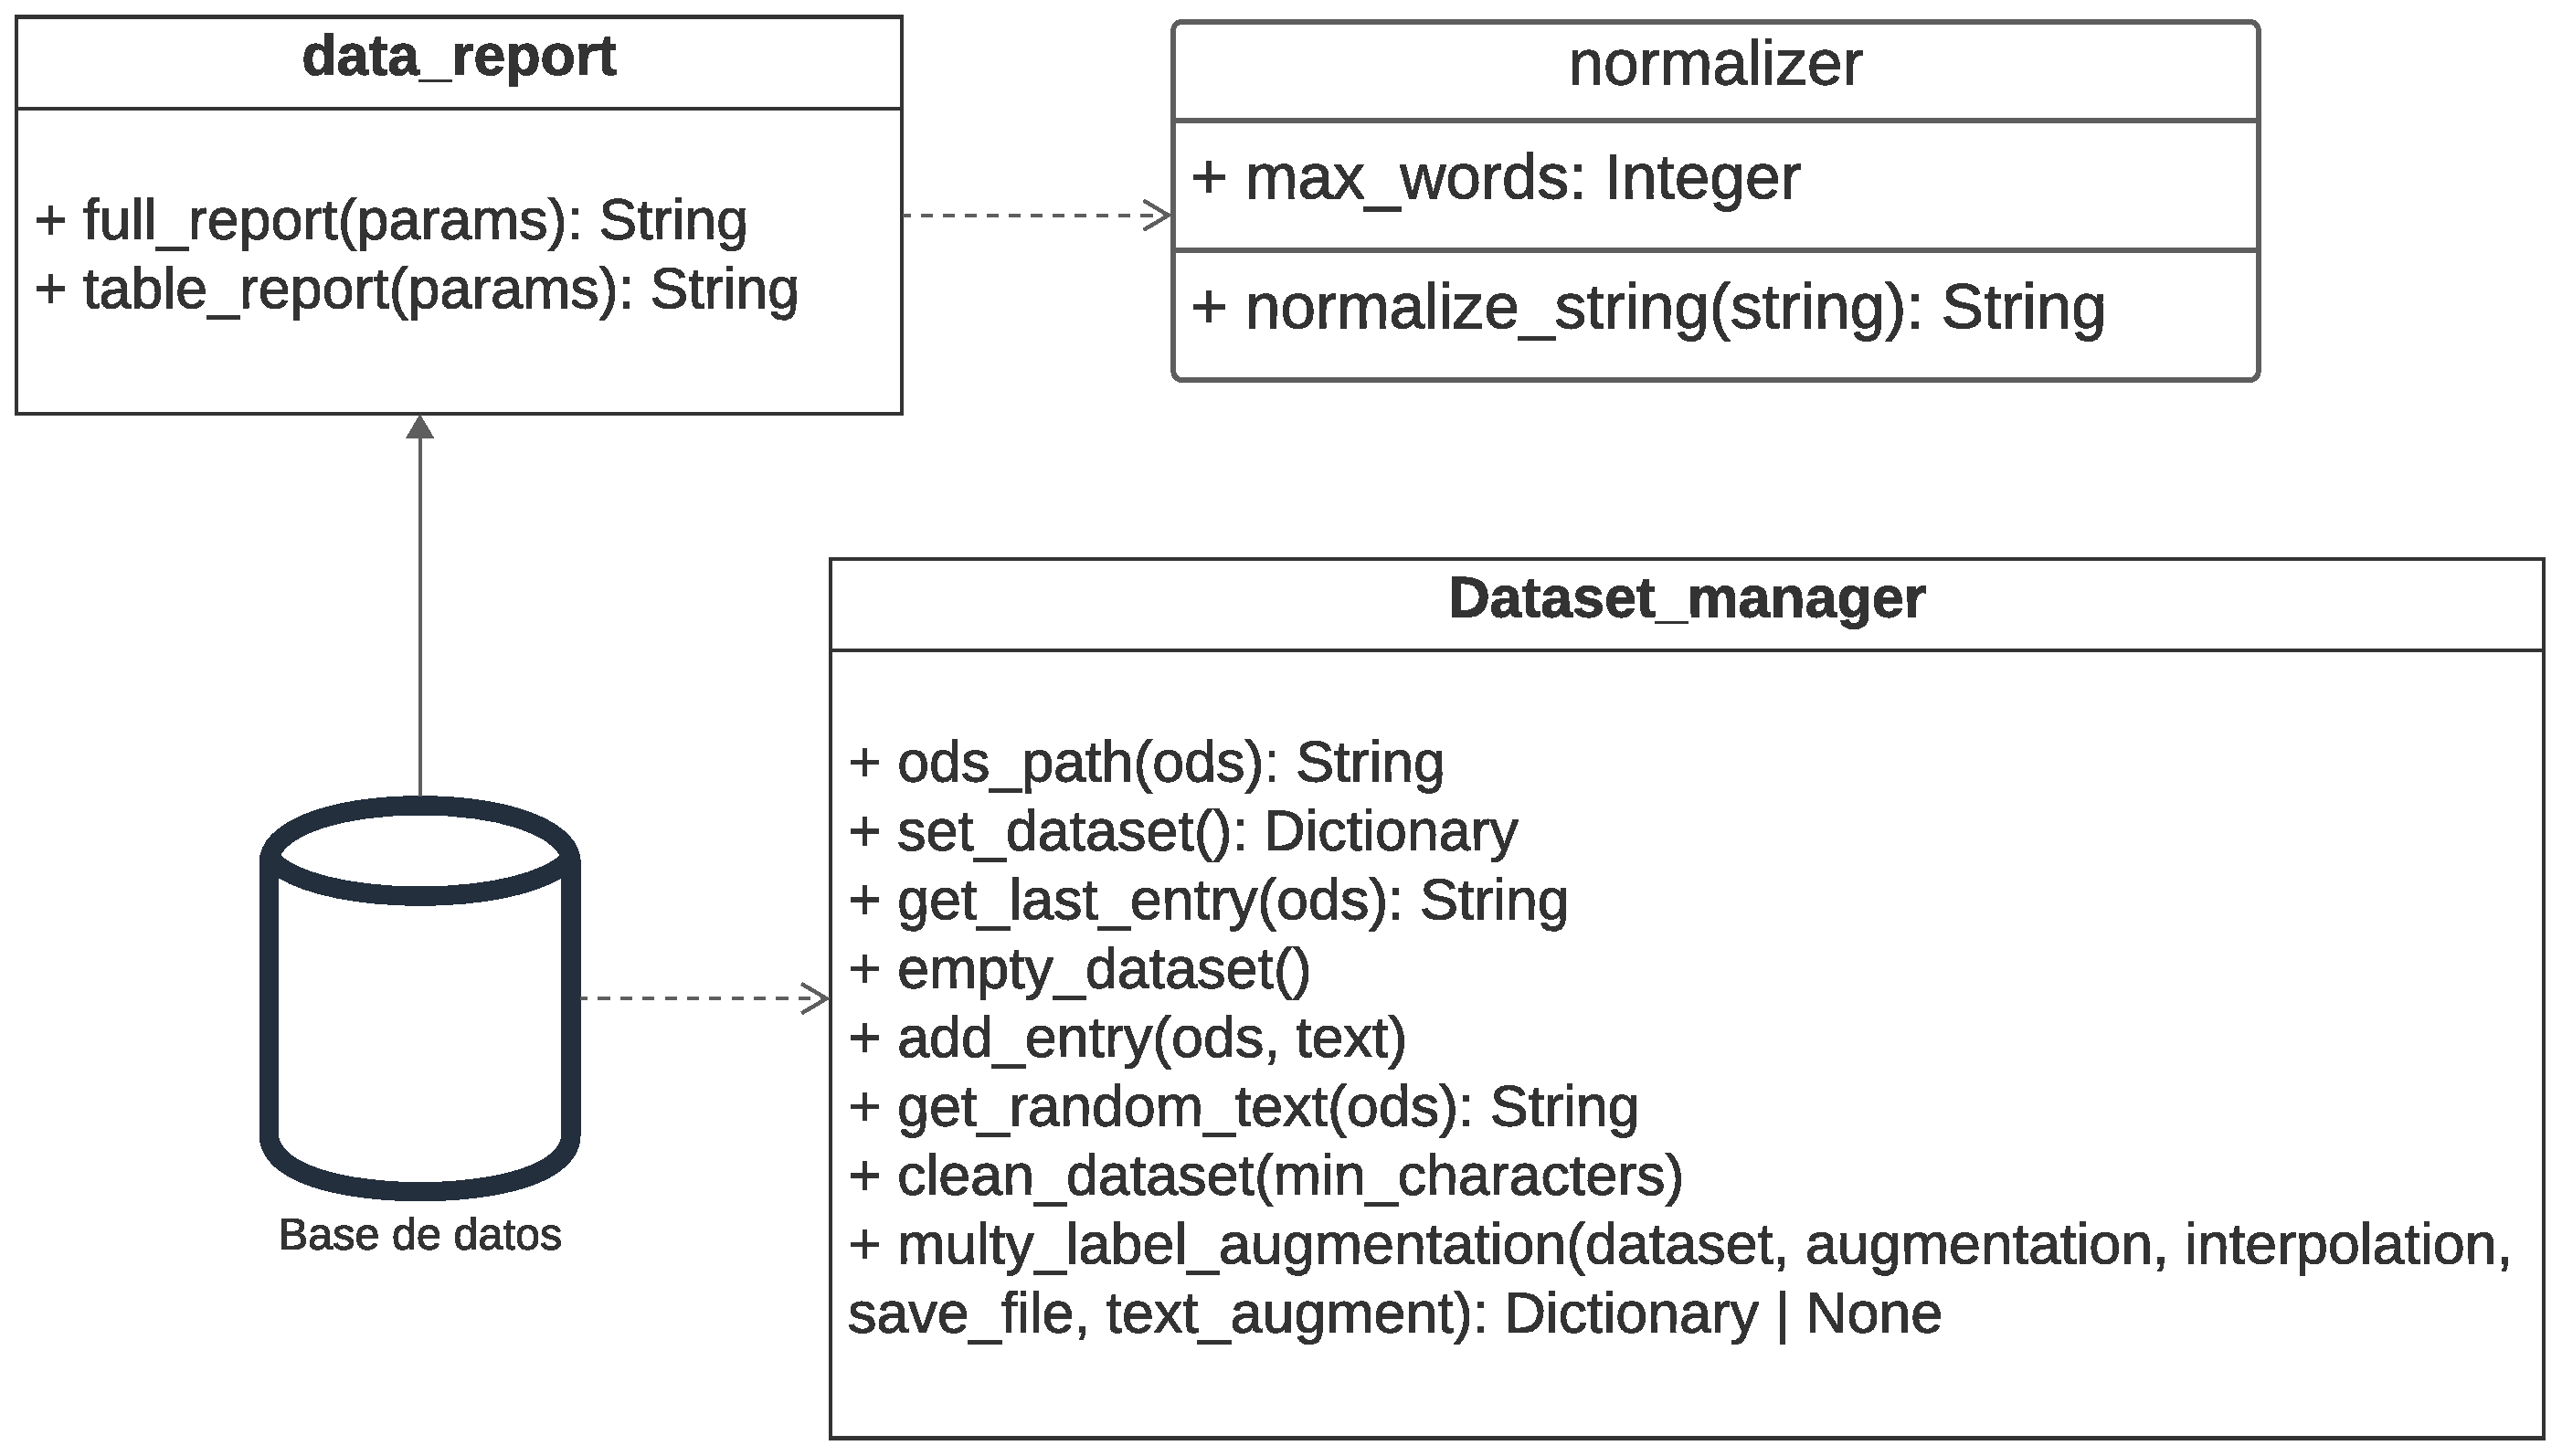
\includegraphics[width=0.9\textwidth]{data_manager}
    \captionsetup{justification=centering}
    \caption{Diagrama UML de la gestión de la base de de datos}
    \label{fig: Diagrama UML de la gestion de la base de de datos}
\end{figure}

\subsubsection{Módulo de gestión de la base de datos} Inicialmente se tenia la
base de datos en forma de directorio, esto resultaba útil por razones explicadas
posteriormente pero tenía limitaciones, una de ella era la gestión de la misma
base de datos, siendo difícil inspeccionar todos los textos, eliminando así los
duplicados y los vacíos. Esta es la funcionalidad que implementa este módulo,
incorporando funciones para la gestión de la base de datos como lo son el
borrado entero de la misma, la limpieza de textos vacíos y repetidos, el añadido
de entradas, la extracción de una entrada aleatoria, la extracción de la última
entrada o el aumento de la misma. Esta última funcionalidad será explicada en
detalle mas adelante.

\subsubsection{Módulo de tratamiento de texto} En este módulo se han implementado dos únicas
funcionalidades pero ambas de alta importancia, una de ellas tienen como
objetivo normalizar le texto a un número límite de caracteres por línea,
haciendo que este sea legible en un archivo normal, esto resulta útil a la hora
de generar un informe de una prueba en la que se incluyen los textos
clasificados. La segunda de las funcionalidades es la de resumir los textos,
esto también es útil a la hora de generar estas mismas salidas, sobre todo
cuando el texto clasificado es muy largo como para poder leerlo rápidamente.

\subsubsection{Módulo de generación de informe} Una vez se ha generado la base de
datos este módulo itera por toda ella para extraer diversas métricas y generar
un informe. Este puede ser de uno de dos tipos, textual y en forma de tabla,
este primero contiene más información pero de una manera más extensa, mientras
que la tabla contiene menos información pero esta es más fácil de digerir.

Ambos tipos de informe cuentan, por cada \gls{ODSa} el número de textos y la
longitud máxima, mínima y media de estos, la única diferencia es la
presentación de estos datos y que en el caso del informe textual se incluyen
textos de ejemplo de cada objetivo. 

\subsection{Gestión de modelos}

\begin{figure}[H]
    \hspace*{-1.7cm}
    \centering
    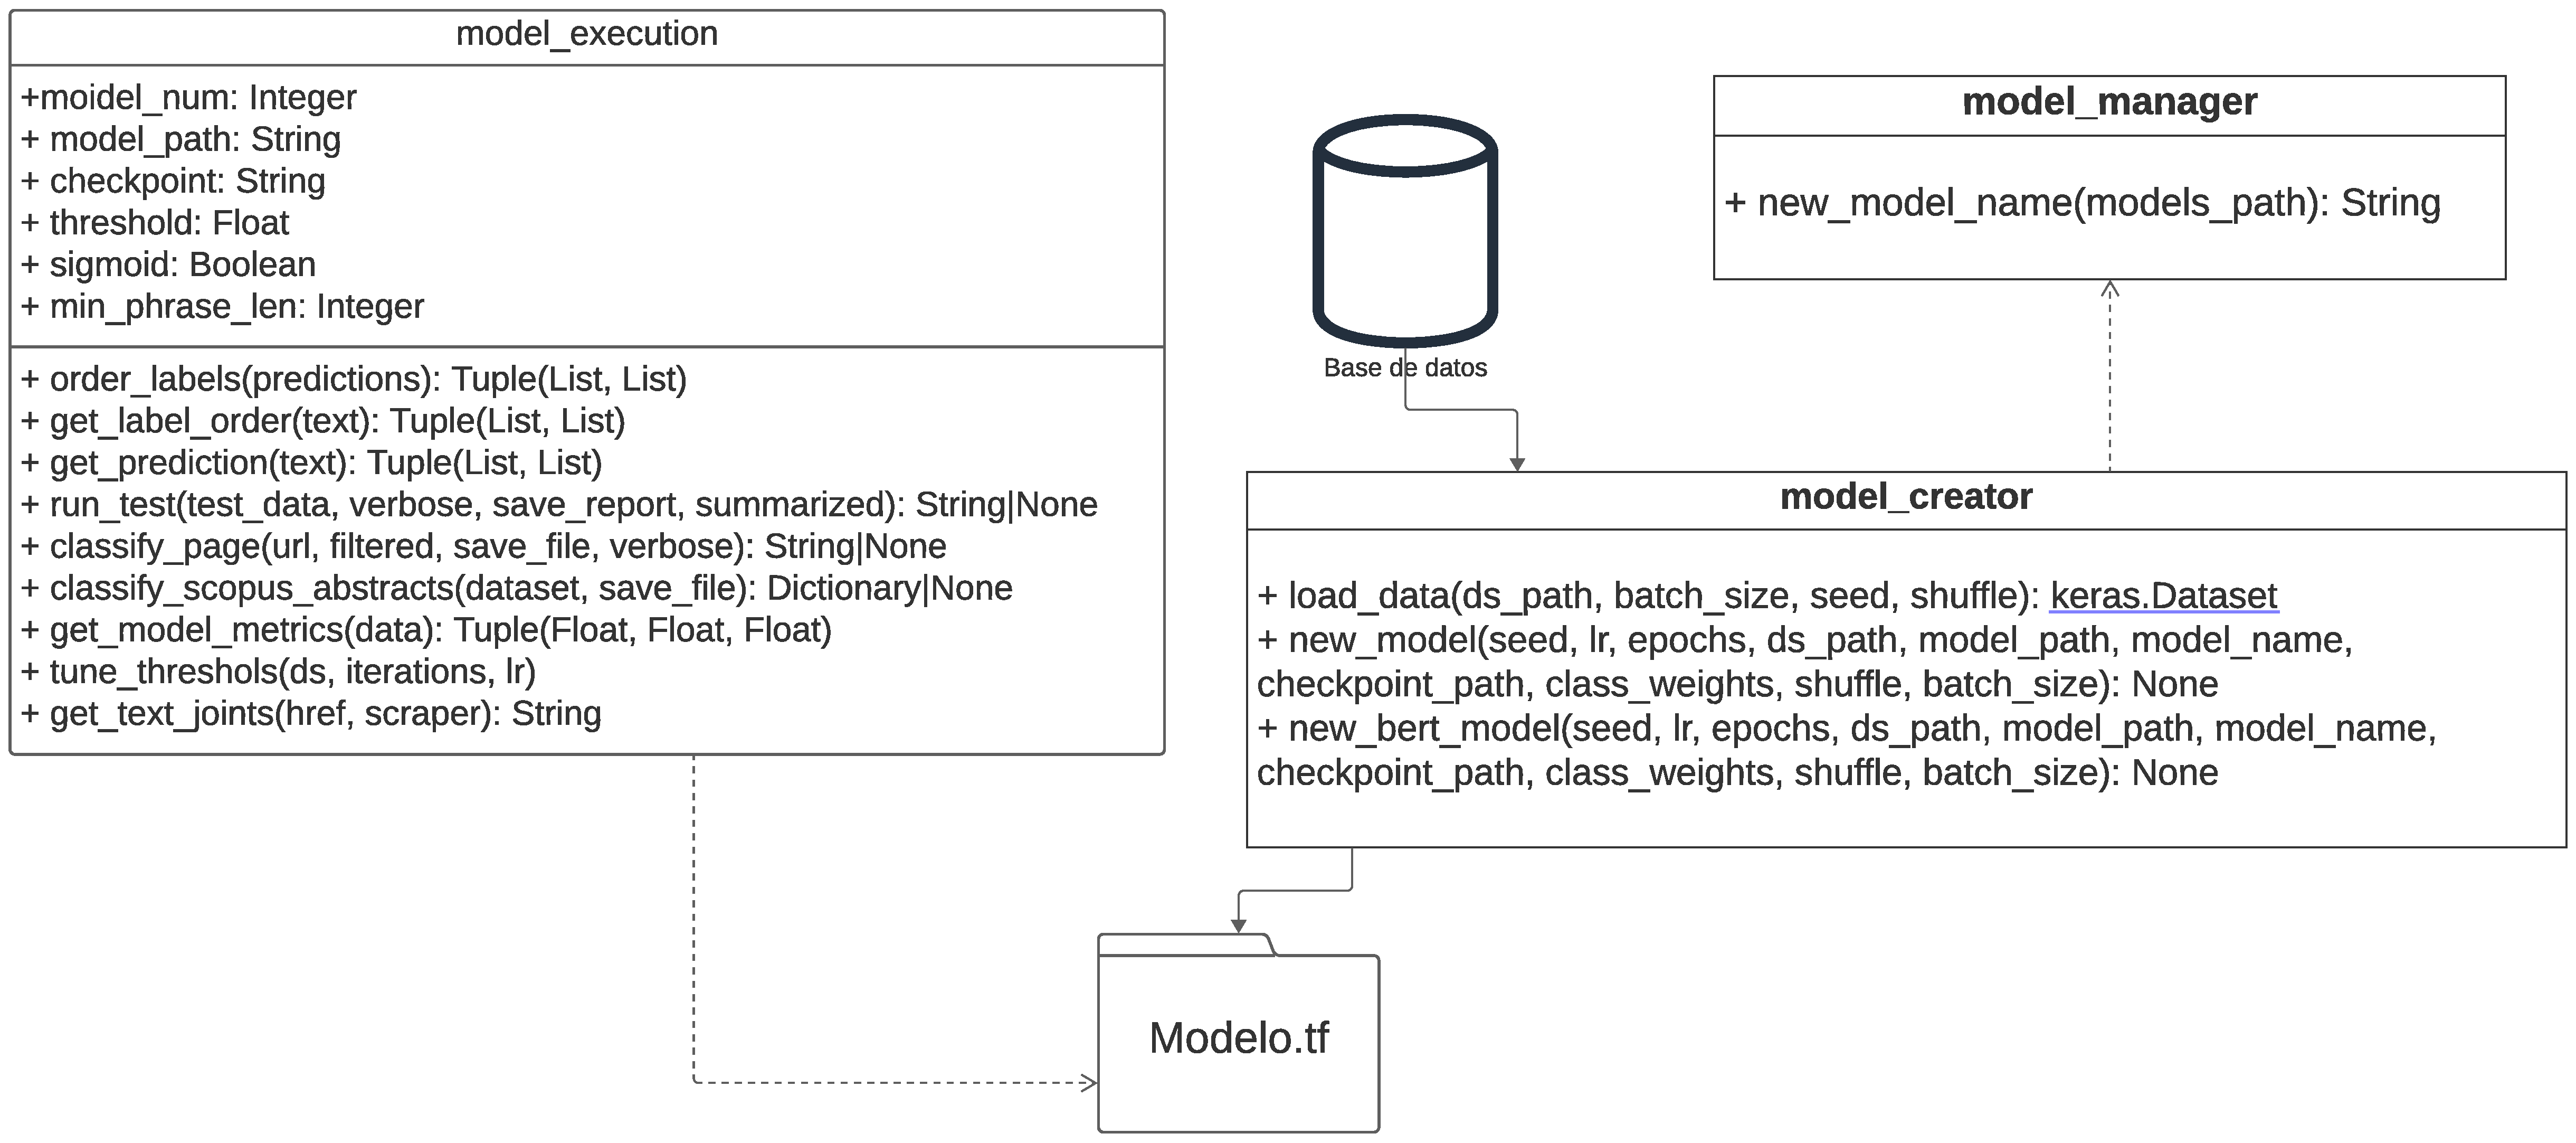
\includegraphics[width=1.2\textwidth]{model_manager}
    \captionsetup{justification=centering}
    \caption{Diagrama UML de la gestión de modelos}
    \label{fig: Diagrama UML de la gestion de modelos}
\end{figure}

\subsubsection{Módulo de creación de modelos} Este módulo es el responsable de
crear, entrenar y validar los modelos. Soporta dos tipos de bases de datos como
entrada, tanto en forma de directorio (explicado más adelante) como en un
\gls{cvsa} y puede crear dos tipos de modelos uno basado en una red
recurrente y otro basado en \gls{BERTa}, en ambos casos se introducen los mismos
parámetros:
 
\begin{itemize}
    \item  Número de ciclos de entrenamiento: número de iteraciones de
    entrenamiento que realizar 
    \item Tasa de aprendizaje: cuánta influencia tienen los
    errores en el entrenamiento, cuanto menor sea el número más ciclos de
    entrenamiento serán necesarios pero este ajustará mejor los pesos. 
    \item  Ubicación de la base de datos: directorio en el que encontrar los
    datos, tanto en forma de directorio como de archivo \gls{cvsa}  
    \item  Ubicación del modelo: directorio en el que guardar el modelo
    entrenado, por defecto se utiliza la regla de nombramiento ``modelXX`` donde
    ``XX`` es el número asociado y existe una función que determina dicho número
    automáticamente por lo que se suele dejar en blanco.  
    \item  Balanceo de clases: indica si se le deben asignar pesos a las clases
    en función del número de ocurrencias de cada una en la base de datos. Esto
    suele resultar en un modelo más uniforme pero puede interferir de manera
    significativa en el entrenamiento. 
    \item  Tipo de arquitectura: atributo utilizado para especificar si crear
    una red recurrente o un modelo basado en \gls{BERTa}.
\end{itemize}
El proceso de creación y entrenamiento es idéntico para ambos modelos, a
excepción de la arquitectura usada, este comienza cargando la base de datos y
dividiéndola en dos conjuntos, uno de entrenamiento y otro de validación,
realizado una división del 70/20. Posteriormente se calcula el balanceo de
clases, si este se ha especificado como activo, y finalmente se entrena el
modelo. En última instancia se guarda el modelo y se utiliza el conjunto de
test para calcular las métricas finales del modelo.

\subsubsection{Módulo de ejecución} Una vez guardado un modelo no es del todo sencillo usarlo
para clasificar textos, sobre todo por la necesidad de interpretar correctamente
las salidas generadas. Este módulo codifica estas funcionalidades para poder
usar los modelos fácilmente. La arquitectura de este módulo consiste en una
única clase que representa un modelo, al instanciar dicha clase se carga el
modelo especificado y se codifican datos necesarios para la ejecución como el
orden de las clases en la salida de los modelos, el tipo de función de
activación usada, el umbral a usar (explicado más adelante) y longitud mínima de
frase. 

Mencionar que las salidas generadas por los modelos tienen una forma de vector
unidimensional con 17 valores entre 0 y 1, uno por cada objetivo. Dicho valor
representa la probabilidad de que ese objetivo esté relacionado con el texto y
puede ser interpretado de diversas maneras dependiendo de la salida usada por el
modelo. La manera en la que se sabe a que objetivo pertenece cada probabilidad
es gracias a que la salida está ordenada siguiendo el orden alfabético de las
clases, por lo que los porcentajes del vector de salida están ordenados de la
siguiente manera [ODS1, ODS10, ODS11, ODS12, ..., ODS17, ODS2, ODS3, …, ODS9]

La clase \textit{model} cuenta con 10 métodos destinados a clasificar textos usando el
modelo indicado e interpretar las salidas generadas, estos son: 

\paragraph{get\_label\_order}
Este primer método es el central de toda la arquitectura, este coge un texto (o
textos)  dado, lo pasa por el modelo asignado y ordena la salida generada de
mayor a menor probabilidad, devolviendo este vector de valores junto con uno
ordenado de igual manera pero sustituyendo los valores por sus respectivos
objetivos.

\paragraph{get\_prediction} Este segundo método encapsula al anterior, haciendo uso de
get\_label\_order para generar los vectores de probabilidades de un texto dardo y
posteriormente interpreta estas salidas para generar la predicción final del
modelo. Dicha interpretación depende de la función de activación presente en el
modelo ya que esta cambia la forma del vector de probabilidades: si esta es
sigmoid al texto se le asignan todos aquellos objetivos cuyos porcentajes
superen el umbral definido al instanciar la clase, en cambio, si la función de
activación de salida es softmax este proceso es menos trivial y será explicado
en un apartado posterior. Finalmente se devuelven los objetivos clasificados por
el modelo con sus respectivas probabilidades.

\paragraph{order\_labels} Éste método no es crucial pero implementa una funcionalidad útil
que se consideró que procedía encapsular en su función. Esta consiste en, dado
un vector de probabilidades, devolver este ordenado de forma descendente junto
con otro vector conteniendo los objetivos ordenados acorde a sus probabilidades. 

\paragraph{run\_test} Método con una funcionalidad sencilla pero útil, dado una base de datos
etiquetada clasificará todos los textos en ella y los comparará, pudiendo
generar un informe en el que se incluyen todos los textos, los objetivos
clasificados y sus porcentajes y finalmente la métrica de precisión total del
modelo sobre ese conjunto de datos.

\paragraph{classify\_page} Una de las funcionalidades más sencillas pero curiosas de las
implementadas es el hecho de clasificar una página web únicamente proporcionando
la url, esto se hace mediante la librería de \textit{requests} y \textit{BeautifulSoup4} pudiendo
extraer todo el texto de una página desde su código fuente.

\paragraph{classify\_scopus\_abstracts} Este método es una primera aproximación de la
funcionalidad final del modelo, clasificar abstracts extraídos de bases de datos académicas como Scopus o \gls{WebOfSciencea}. Este extrae los abstracts de un \gls{cvsa}, los
clasifica todos y genera como salida el número de textos asignados a cada
objetivo.

\paragraph{tune\_threshold} Más adelante se explicará en detalle el uso de umbrales,
explicado superficialmente se usan para decidir qué etiquetas se asignan al
texto y cuáles no en base a los porcentajes generados por el modelo. Este valor
del umbral necesita ser ajustado y es por esto que por medio de un gran número
de datos de prueba y calculando las métricas usando get\_model\_metrics para un
alto número de valores del umbral se pueden identificar tendencias y relaciones
entre las métricas y el valor del umbral, pudiendo así, decidir el valor óptimo
de este.

\paragraph{get\_text\_joints} Como añadido se definió este método que extrae texto de
artículos de una determinada página, \textit{jointsdgfound} \cite{JointSDGFund}, esto se hizo debido a
que se tenía un gran número de enlaces a artículos de esta página clasificados
con sus respectivos objetivos por lo que para clasificarlos mejor se optó por
escribir este método, de esta manera se podían usar estos textos como conjunto
preliminar de prueba.

\subsubsection{Módulo gestor de modelos} Éste módulo se creo con la expectativa de una necesidad
de gestionar los modelos mayor de la que finalmente resultó ser necesaria, es
por esto que cuenta con una única función, el cálculo del nombre del siguiente
modelo a entrenar, anteriormente se ha explicado que el nombre de los modelos
siguen el patrón ``modelXX`` donde ``XX`` es un número que los identifica, esta función
lee los modelos existentes y calcula cual es el siguiente número disponible para
asignar.


\section{Desarrollo realizado}Anteriormente se han definido todos los modelos
desarrollados pero no como estos fueron creados. Es este apartado se describirá el proceso de
desarrollo seguido, como todas las partes interactúan y su papel en el sistema.

Para empezar cualquier trabajo de aprendizaje automático es fundamental contar
con una buena base de datos ya que es de esta de la que se va a extraer el
conocimiento a usar en el futuro. Esto se suele solucionar fácilmente buscando
una base de datos disponible en internet o, hasta en algunos casos, generándola
automáticamente de manera local. En este caso, después de una extensa
investigación no se encontró ninguna base de datos existente con textos
etiquetados de acorde a los objetivos de desarrollo sostenible. Descartando esta
opción, la última alternativa disponible es generar esta base de datos de manera
manual o pseudo-manual, en este caso se optó por utilizar técnicas de \textit{Web
Scraping} para extraer textos de páginas que contenían información segmentada
acorde a los \gls{ODSa}. 

Como primer recurso se acudió a la propia página de
las naciones unidas para guardar las definiciones y metas de cada objetivo, esto
probó ser una tarea imposible ya que esta información no se almacena de manera
textual en la propia página si no que se encuentra codificada dentro de una
serie de imágenes. Si se hubiera investigado mas seguramente existiera tal
información almacenada de manera textual y accesible. Tratándose de textos
comunes se consideró que lo más sencillo era buscar una segunda fuente, aquí es
donde se encontró la página de \textit{jointsdgfound} \cite{JointSDGFund}, esta contiene las
definiciones, metas e información adicional sobre cada objetivo de una manera
ordenada en la propia página por lo que su extracción y etiquetado fueron tarea
sencilla. Se extrajeron un total de 187 entradas, idealmente 11 por cada clase,
pero los datos presentan una distribución altamente desbalanceada, siendo el que
más textos asignados tiene el objetivo 17 con 20 datos y los que menos el 7 y 13
con 6. 

Investigando se encontró un repositorio en esta misma página \cite{JointSDGFund}
conteniendo multitud de artículos, estando estos etiquetados con los objetivos
sobre los que se habla. Dichos artículos se catalogaron, almacenando sus
direcciones junto con los objetivos relacionados. Después de analizar estos
datos nuevos se vio que la mayoría de ellos estaban relacionados con demasiados
objetivos como para poder usarse para identificar las diferencias entre ellos.
Debido a esto no se usaron para entrenar ningún modelo pero si se almacenó la
información recolectada para posteriormente usarse como una prueba más que
realizar con los modelos. 

Una vez recolectados los datos, se diseño un modelo de una red recurrente. Se
eligió este tipo de arquitectura debido a su potencia a la hora de tratar con
datos secuenciales, como lo son los textos. La arquitectura final del modelo
implementado se basó en uno publicado por los desarrolladores de tensorflow,
contando este con una serie de capas recurrentes conectadas a una red prealimentada. El resto de
parámetros se eligieron en función del problema a resolver, la función de
activación usada fue softmax, y como optimizador se eligió \gls{ADAMg} (\gls{ADAMa}), debido principalmente a su capacidad de adaptar la tasa de aprendizaje dependiendo del tipo de aprendizaje que se esté haciendo, y a que es ampliamente utilizado en tareas de aprendizaje automático debido a su versatilidad y potencia.

Una vez diseñado un modelo, este se entrenó usando los datos extraídos
inicialmente. Este modelo primordial probó ser insatisfactorio (las métricas
obtenidas se presentarán más adelante). Se conseguían unas métricas excelentes
en el conjunto de entrenamiento de una manera muy rápida, mientras que las
métricas del conjunto de validación se mantenían estables en un rango muy por
debajo del aceptable. Este es un problema clásico de sobreaprendizaje, causado
habitualmente por una falta de datos de entrenamiento. 

Debido a estos resultados se buscó encontrar nuevas entradas, estas al final se
extrajeron de los informes publicados anualmente por la \gls{ONUg}. Se tomó
esta decisión ya que estos informes están segmentados por año y por objetivo,
haciendo fácil su extracción cambiando la fecha en la dirección web, y su
etiquetado, estando estos ya clasificados. La base de datos se aumentó hasta un
total de 1118 entradas ya que se decidió dividir los informes por cada punto y
añadir cada segmento resultante de manera independiente a la base de datos. De
este modo se consiguió un conjunto de datos mucho más extenso y completo, y más
importante aún bastante balanceado, con la única excepción del objetivo 17 ya
que este cuenta con 120 entradas mientras el resto cuenta con alrededor de 60
cada uno. 

Con estos nuevos textos añadidos se consiguieron los primeros resultados
aceptables, siendo este un modelo bastante capaz, consiguiendo clasificar
correctamente la mayoría de los casos y hasta razonando objetivos que no estaban
asignados a los textos y que si tenían sentido clasificarse de esa manera. Este modelo, aunque no especialmente potente,
sirvió como precedente, demostrando que si era posible diferenciar correctamente
los objetivos y que los datos usados eran de cierta calidad.

De todas formas no era un modelo suficientemente capaz como para usarlo para
realizar un estudio cuantitativo de una manera fiable, es por esto por lo que se
decidió variar la arquitectura usada y entrenar modelos basados en
\gls{BERTa}. Para esto se hizo uso de la librería tensorflow-hub la cual
permite a los desarrolladores descargarse modelos preentrenados y adaptarlos a
sus necesidades. Ese modelo descargado está formado por una parte principal,
esta, llamada \textit{codificador}, emplea mecanismos de atención para codificar
las entradas textuales, es en esta parte donde se asignan las importancias a las
palabras y sus relaciones. Es por esto por lo que es necesario añadir una capa
adicional que sea capaz de decodificar estás codificaciones para generar las
salidas esperadas. 
% una encargada de codificar las entradas textuales y otra que se encarga de
% aplicar el conocimiento almacenado para generar las salidas. implementa los
% mecanismos de atención usados para inferir las relaciones entre las palabras
% para poder entender el texto y generar la salida deseada. 

Aquí es donde se empezó a conseguir modelos realmente potentes, estos consiguen
clasificar correctamente casi todos los textos y razonar objetivos nuevos con
mucho más criterio. Esta última faceta es la más llamativa ya que inspeccionando
las salidas se veía como el modelo era capaz de entender los textos de una
manera profunda, interpretando patrones aún más complejos y clasificando
objetivos nuevos a datos ya etiquetados con mucho más criterio.


%-----------------------------------------------------------------------------
%-----------------------------------------------------------------------------
Fue llegado este punto en el que se decidió implementar una clasificación
multi-etiqueta, hasta hora el conjunto de datos de entrenamiento y de pruebas
constaban de textos que tenían asignado únicamente un objetivo, \textit{one-hot}
y en la interpretación de las salidas solo se tenía en cuenta el objetivo con mayor
porcentaje asignado. 

Aquí se enfrentó uno de los principales problemas encontrados en el desarrollo,
la función de activación de salida usada hasta ahora era softmax, esta era la
decisión correcta debido al formato de los datos, pero resultaba ser un problema
a la hora de implementar esta nueva funcionalidad.

Como solución se decidió implementar una nueva forma de interpretar las salidas.
Esta es similar a la que se utiliza con redes con función de activación sigmoid,
en este caso se asignan todas las clases  cuyo porcentaje supere un umbral. La
técnica implementada es similar ya que asignan todas las clases que superen un
umbral, la diferencia clave está en la definición de dicho umbral.

En el caso de las redes con función de activación sigmoid simplemente se define
un porcentaje mínimo a usar como umbral. En el caso de la función softmax esta
solución no resultaría muy efectiva ya que la magnitud de los porcentajes
generados varía ampliamente debido a su naturaleza aditiva. Esto hace que en los
casos en los que haya muchos objetivos relacionados con un texto, la
probabilidad estará distribuida entre muchas clases, siendo esta relativamente
baja en todas pero, en un caso ideal, relativamente similar en magnitud entre
todas las clases relacionadas. El caso opuesto no resultaría en un problema ya
que si solo hay un objetivo relacionado el porcentaje de este será alto mientras
que la probabilidad restante estará dividida entre el resto de clases. 

Son estas características las que se aprovechan en esta nueva técnica, en esta
se define un umbral inicial, este, una vez se obtienen las probabilidades
generadas por el modelo su multiplica por la mayor de todas, de esta manera se
genera un umbral adaptado al dato de entrada. Si este está relacionado con
diversos objetivos y se genera un vector con probabilidades similares entre
varias clases, estas serán similares en magnitud pero pequeñas, generando, a su
vez un umbral final bajo, consiguiendo así clasificarlas. Por otra parte si el
texto solo está relacionado con un objetivo, o es uno muy dominante, este
obtendrá un porcentaje asignado alto por lo que no se asignarán más objetivos. 

% que se usará para calcular el umbral definitivo que
% se usará en las comprobaciones, esto se hace multiplicando l


% esto es un problema si se quiere
% realizar una clasificación multietiqueta pero es la adecuada si se cuenta con
% datos con una única clase asignada. Para solucionar esto se decidió implementar
% una variable de la clasificación top-p [FUENTE]. En este tipo de clasificación
% se toma la salida genereada por la red y se asignan los aquellas clases cuyos
% porcentajes sumen más que un umbral determinado. Esta estrategia se consideró
% inadecuada y se modificó de la siguiente manera para adaptarla: se utilizaba un
% umbral de misma manera que al usar una función de activación softmax, todas
% aquellas clases cuyos porcentajes sean mayores al umbral son asignadas a la
% entrada, en este caso se hizo algo parecido pero el umbral en vez de ser un
% valor fijo está en proporción al porcentaje mayor asignado por el modelo, de
% esta manera, si la salida generada es un vector como este [0.3, 0.25, 0.18,
% 0.04,...] se usará como umbral 0.3 multiplicado por un determinado porcentaje, y
% todas aquellas clases cuyos porcentajes sean superiores a ese número serán
% asignadas. Se decidió interpretar las salidas de esta forma debido a que todos
% los porcentajes suman 100%, por lo que si se define un umbral fijo alto, en
% aquellos casos en los que se espera que el modelo asigne más de una etiqueta, la
% clasificación no se realizará correctamente puesto que la naturaleza aditiva de
% la función de activación hace que no todas las clases relacionadas puedan tener
% un porcentaje alto. Lo contrario también es cierto puesto que si se espera que
% el modelo clasifique solo una etiqueta esta puede no tener un porcentaje
% asociado muy alto y si el umbral es bajo se asignarán etiquetas erroneas. Es por
% esto por lo que se decidió asignar un umbral relativo, si el texto dado tiene
% muchos objetivos asociados se espera que todos estos porcentajes sean
% relativamente bajos y de valor parecido, por lo que el umbral será menor y se
% clasificarán mas objetivos, pro otra parte si el texto solo tiene un objetivo
% relacionado se espera que el porcentaje asociado de este sea relativamente alto
% por lo que el umbral tambien será elevado, siendo más difícil clasificar
% objetivos poco relacionados. La única dificultad en este proceso está en
% calcular por cuanto multiplicar el porcentaje más alto para obtener el umbral,
% esto es un proceso que se explicará más adelante. 
%-----------------------------------------------------------------------------
%-----------------------------------------------------------------------------

Esta funcionalidad resultó funcionar según lo esperado, clasificaba
correctamente más de un objetivo en algunos casos, pero se vio que era
imprescindible realizar un buen ajuste del umbral (De aquí en adelante se
utilizará umbral para referirse al porcentaje por el cual se multiplica la
probabilidad mayor para obtener el umbral de verdad) ya que es necesario
encontrar un buen valor para realizar una buena clasificación.

Es aquí donde se llegó a uno de los puntos de inflexión, se consideró terminar
el desarrollo, con un buen modelo clasificador y adaptado para realizar una
clasificación multi-etiqueta pero el método usado, al ser una variación  de
otro, no resultaba cómodo de usar como modelo final. Después de investigar se
decidió realizar la clasificación multi-etiqueta de una manera mas aceptada y
probada. Haciendo uso de una función de activación de salida sigmoid. Esta
función, como se explicó en el estado de la cuestión, genera un vector de
probabilidades independientes por lo que se pueden asignar todas aquellas que
superen un porcentaje determinado, denominado umbral. 

Se entrenó un nuevo modelo con los datos ya existentes, pero al no tener estos
una forma adecuada no se obtuvieron resultados diferentes a los que se consiguieron  con el
modelo anterior. Esto es debido a que todos los datos tienen un único objetivo
asignado, no hay ningún texto con más de un objetivo asociado por lo que,
independientemente del tipo de arquitectura y función de activación usada, el
modelo no va a ser capaz de clasificar más de un objetivo porque no es un caso
al que haya sido expuesto previamente.

Esto es algo que se pensó solucionar a posteriori, a la hora de clasificar un
texto más grande dividir este en sus diferentes frases, para posteriormente usar
un modelo especializado en identificar objetivos uno a la vez y en frases cortas
para clasificar cada una de manera independiente y finalmente realizar la media
de los porcentajes generados para cada una. De esta manera si se habla de más de
un objetivo esto se verá reflejado en alguna frase, teniendo un impacto en los
porcentajes finales y, si todo funciona según lo esperado, clasificando el texto
correctamente. Esto probó no merecer la pena, por un lado, dividir un texto en
sus frases y clasificarlas independientemente resulta tener un impacto
significativo en el rendimiento, tardando bastante más que clasificando textos
enteros. Por otro lado analizando los textos con los que se va a usar el modelo
final, textos científicos cortos (abstracts), se vió que resultaría más útil
generar un modelo capaz de clasificar correctamente textos enteros que las
diferentes frases, ya que estos textos suelen tener menos información y esta
está más repartida. Adicionalmente, de esta manera también se aprovecha la
naturaleza bidireccional de los modelos basados en BERT. Es por esto que se
decidió generar una base de datos con múltiples etiquetas.

% Inicialmente se varió únicamente esta función de activación pero los datos al no
% tener una forma adecuada, cada dato de ejemplo solo esta asociado a una
% etiqueta, resultaba en un modelo similar al anterior. Se consideró buscar más
% datos para introducirlos al conjunto de entrenamiento pero finalmente esa idea
% se descarto a favor de otra más sencilla explicada a continuación.

Para conseguir  generar una base de datos multi-etiqueta se hizo uso de una
técnica muy común en el aprendizaje automático, el aumento de datos,
aplicándola de una manera particular. Esta técnica consiste en generar datos
nuevos a partir de unos ya existentes, variando sutilmente estos mismos de tal
manera que son datos diferentes pero no lo suficiente como para que su etiqueta
asociada ya no tenga sentido. Esta técnica es usada en multitud de problemas, el
más llamativo de todos siendo en el uso de imágenes, pudiendo rotar, desplazar,
recortar o hasta alterar los colores de la imagen sin que esta pierda su
sentido. Cuando se trata con datos textuales existen multitud de formas de
aumentar estos datos, una serie de ellos se demonima \gls{EDAg} (\gls{EDAa}), aumento de datos sencillo. Esta serie
de algoritmos realiza operaciones como sustituir palabras por sinónimos,
eliminar palabras aleatorias, cambiar de posición una serie de palabras de
manera aleatoria. Adicionalmente existen una serie de métodos algo más
sofisticados como son:

\begin{itemize}
    \item Wordnet: Este es el nombre de uno de los modelos de vectorización de
    texto mas potentes, este se usa para aumentar la base de datos de manera
    similar a cuando se reemplazan palabras con sus sinónimos pero en vez de
    elegir estos sinónimos en base a una base de datos estás palabras sinónimas
    son aquellas que se encuentran próximas a la palabra objetivo en este
    espacio vectorial, de esta manera, a ojos del modelo las palabras no serán
    las mismas pero su significado si será parecido. 
    \item Traductor: Este tipo de aumento es muy curioso pero útil a la vez.
    Este se basa en algo que todo el mundo ha hecho, escribir una frase en un
    idioma, traducirla a otro cualquiera y volver a traducir esa frase al idioma
    original. El resultado rara vez es la misma frase pero el significado sigue siendo el mismo en la mayoría de los casos. Este tipo de aumento
    hace uso de este proceso para traducir la frase a un idioma determinado y
    luego de vuelta al original, de esta manera obtendremos dos frases
    diferentes pertenecientes a la misma etiqueta.
\end{itemize}

Esta técnica de aumento se usó para generar un nuevo conjunto de datos
multi-etiquetados partiendo de los anteriores. Como técnica de aumento a usar se
escogió Wordnet. Este aumento consistió en elegir de entre 2 y 5 textos, cada
uno de un objetivo diferente, estos textos se transformaron usando Wordnet y se
juntaron en una entrada nueva, estando esta etiquetada con los objetivos de los
textos seleccionados. De esta manera se aumentó la base de datos a un total de
más de 5000 entradas. 

Con este nuevo conjunto de datos se entrenó un nuevo modelo, el cual rindió mejor que los anteriores en tareas de clasificación multi-etiqueta. 

Finalmente, investigando trabajos similares se descubrió una página que contaba
con una gran cantidad de artículos relacionados con los objetivos de desarrollo
sostenible, en la mayoría de los casos con mas de uno a la vez, el \textit{\gls{IISDg} }(\gls{IISDa})
\cite{IISDHomepage}. Después de examinar estas publicaciones se vio que eran
de una buena calidad, y contaban con el aval de haber sido usadas en trabajos
similares. Fue por estas razones por la que se decidió generar un último
conjunto de datos, no tan grande como el generado con técnicas de aumento de
datos, pero de mayor calidad. Se desarrolló un último script de extracción de
datos que recogía los enlaces y otro que extraía los textos de dichos enlaces y
los guardaba con sus respectivas etiquetas. Fue en este momento cuando se
llevó a cabo una transición de una base de datos en forma de directorio a una en un
archivo \gls{cvsa}, ya que la naturaleza multi-etiqueta hace que esta última sea la
mejor opción. 

Como último añadido se vio que la página del \gls{UNDPg} (\gls{UNDPa}) \cite{UNDPHomepage} contenía
definiciones diferentes y extensas de los objetivos por lo que también se
añadieron a la base de datos

Se desarrollaron dos últimos grupos de modelos, unos entrenados únicamente con
los datos extraídos de las publicaciones de \gls{IISDa} y
otros finales desarrollados con el conjunto final, contando con los datos
extraídos al inicio (las definiciones y los informes publicados por naciones
unidas) y estas últimas dos extracciones. De este último conjunto se dejaron
fuera los datos creados mediante técnicas de aumento ya que se consideró que el
tamaño de este era suficiente y se priorizó la calidad de los datos. 

Estos últimos modelos son los que mejores resultados obtuvieron, no en magnitud
de algunas métricas si no en el equilibrio de estas, obteniendo buenos
resultados en todas. 

Finalmente se utilizó el modelo para realizar una investigación del contenido de
las publicaciones científicas publicadas, esta investigación se cubrirá en
detalle en apartados posteriores. 

